                                                                                                                        \documentclass{article}
\usepackage{graphicx} % Required for inserting images
%\usepackage{subtitle}
\usepackage{titling}
\usepackage{xcolor}
\usepackage{hyperref}
\usepackage{lmodern}
\setlength{\parindent}{0pt}
\usepackage{listings} %I need this for the code; Leonie
\usepackage[utf8]{inputenc}

% stuff for image centering, multiple images, etc.
\usepackage{float}
\usepackage{lipsum}
\usepackage{mwe}


%Updated the margin on the side... [also the code looks better]
\usepackage[a4paper, margin=2.5cm]{geometry}


\pretitle{%
  \begin{center}
  \end{center}
  \Huge\bfseries
  \textcolor{blue!70!black}{\rule{\textwidth}{1pt}}\\[\bigskipamount]
}
\posttitle{%
  \\[\bigskipamount]
  \Large\textit{Controversies in Game Theory FS25}\\[1em]
  \textcolor{blue!70!black}{\rule{\textwidth}{1pt}}\\[\bigskipamount]
  \end{center}
}
\preauthor{%
  \begin{center}
  \large
}
\postauthor{\end{center}}
\predate{%
  \begin{center}
  \large
}
\postdate{\end{center}}

%Brauche ich ebenfalls für den CODE :)) Leonie

\definecolor{codegreen}{rgb}{0,0.6,0}
\definecolor{codegray}{rgb}{0.5,0.5,0.5}
\definecolor{codepurple}{rgb}{0.58,0,0.82}
\definecolor{backcolour}{rgb}{0.95,0.95,0.92}

\lstdefinestyle{mystyle}{
  language=Python,           % Programmiersprache
  basicstyle=\ttfamily\footnotesize, % Schriftart
  backgroundcolor=\color{backcolour},   %Hintergrund
  commentstyle=\color{codegreen}, %Kommentare
  stringstyle=\color{codepurple}, %Strings
  keywordstyle=\color{magenta}, % Keywords
  numbers=left,              % Zeilennummern
  numberstyle=\tiny\color{codegray},
  stepnumber=1,
  numbersep=10pt,
  backgroundcolor=\color{gray!10},
  % frame=single,              % Rahmen um den Code
  breaklines=true,           % Zeilen umbrechen
  breakatwhitespace=false,  
  showtabs=false, 
  showstringspaces=false,
  showspaces=false,
  tabsize=2,
  captionpos=b,                    
  keepspaces=true,                 
  numbers=left,
  numbersep=5pt,
}

\lstset{style=mystyle}



\begin{document}

\begin{titlepage}
    
\makebox[0pt][r]{%
  \raisebox{2.5cm}[0pt][0pt]{\hspace{-1.5cm}%
    
\includegraphics[width=0.25\textwidth]{eth_logo_kurz_pos.png}%
  }%
}
  
  \centering
  \vspace*{2cm}  % Adjust vertical top spacing
  {\fontsize{22pt}{28pt}\selectfont\bfseries
  Game Theory and the Dead Internet Theory:\par}
  \vspace{0.1cm}
  {\fontsize{20pt}{26pt}\selectfont\bfseries
  Interaction between Bots and Humans on the Web\par}

  \vspace{1.5cm}
  {\Large\itshape Controversies in Game Theory FS25\par}

  \vspace{2cm}
  \rule{\textwidth}{1pt}

  \vspace{2.5cm}
  {

    June 2025\par
  }

\end{titlepage}

    
\newpage

\section{Introduction} 
In recent years, an increasingly discussed idea has gained attention online — the Dead Internet Theory. The Dead Internet theory is a conspiracy theory which states that the Internet now consists mainly of bot activity and automatically generated content. It has two components: that human activity on the web has been replaced by algorithmically selected search results supervised by AI, and that the government is doing this to manipulate society. In this paper, we will focus more on the first part. This theory has gained more and more believers throughout the world in the last few years, as social media platforms have become the most popular form of news and information. Similar theories such as the Illuminati theory are also widely known. \cite{wikipedia_dead_internet} We believe that if the Dead Internet Theory were to take place, trust in online interaction would worsen, as users would become more uncertain whether they are engaging with a person, a bot, or a cleverly trained AI agent.\\

Authenticity plays a key role in this scenario. Humans must signal their identity in ways that are credible, while bots try to mimic these signals to pass as genuine, with the objective of retaining the human's attention. But we people don't want to interact with fake news and posts, but preferably seek authentic and entertaining content that satisfies our needs. This interaction between humans and bots is what we call the Authenticity Signal Game, which we will look at in more detail throughout this report. Further, three domains of game theory (classical, evolutional, and behavioural) will be inspected and discussed in context with the Dead Internet Theory. \\
This topic is especially important for the future of social networks. One can visualize possible outcomes and different futures (dystopian or utopian) by simulating a signalling game and letting it run for many cycles.

The goal of this project is to find a good equilibrium within this game, where authentic content thrives and to look at what needs to be done for that to happen. Possibly to achieve this equilibrium, it may require external influences such as technology or policy. But we will mostly look at the analytical results of our simulations and some theoretical ideas within game theory.


\newpage

\section{Game Theory and the Dead Internet Theory} 
%By tanish the banish father of the radish: he is very mannish, and possibly danish, but speaks fluently spanish. He will vanish if you try to planish his germanish, romanish fannysh. (by Aaron Cronin)

% By Tanish the Banish, father of the Radish,
% He is very Mannish, and possibly Danish,
% But speaks fluent Spanish — with flair that's outlandish.
% He’ll vanish if you planish his Germanish fannysh,
% And brandish his sword if you’re acting too clownish.

% He’s lavish, not famish, his style never vanish.
% He’ll tarnish your garish, outlandish varnish.
% He once met a granish who spoke only Yiddish,
% Then danced with a banish from old-world Finnish.

% He’s swankish and brackish, a bit devil-may-care-ish,
% His boots are outlandish, his cape quite squeamish.
% He doesn’t like blandish or anything squeamish,
% And won’t eat a dish if it looks too delish.
% by chatgpt (of course)

\subsection{Classical Game Theory}
In Game Theory, the dynamics and implications of the Dead Internet Theory have multiple intersections with it's domain. In classical game theory, the foundational domain, the focus is placed on analyzing rational decision-makers and their strategies usually leading to a conflict of interest \cite{game_theory_definition}. Rationality in the context of game theory in general is a highly debated, almost enigmatic concept \cite{rationality_game_theory}; however, for this report we will simplify it to the following: The act of a person or a party of choosing a strategy that maximizes their own payoff given the other people's or parties' strategy/strategies. \\

There are 2 main actors in the case of the Dead Internet Theory: 1. Human users and 2. AI/Bot operators. While both are assumed to be rational, they have conflicting interests. Humans utility include authentic information, meaningful social connection, entertainment, etc., whereas bots objectives may range from maximizing engagement metrics for revenue, misinformation or controlling/spreading narratives (as per the Dead Internet Theory).\\
A Nash Equilibrium is a state where no player can improve their payoff by changing their own strategy, whilst all other players maintain their strategy. It is a stable point where everyone is doing their best response \cite{green_beards}.  This concept will be elaborated further.\\

Although classical game theory provides a useful "framework" for analyzing situations, the complexity of interactions \& dynamics between both actors in the Dead Internet Theory is heavily abstracted, which is why we consider the problem in other domains as well.

\subsection{Evolutional Game Theory}
In evolutionary game theory \cite{EGT_slides}, strategies are not consciously chosen by individuals but rather traits of behaviours that are "inherited" either genetically or culturally, and whose prevalence changes based on their success. As such, strategies of both players align with their objectives. While from an evolutionary standpoint these may not have been relevant a few decades back, humans in the digital age may pursue "seeking authenticity", "engaging with superficial content" (for example through doom-scrolling), or even simply "disengaging from online platforms" entirely. While a bots strategy might not be entirely evident, we consider the strategies "mimicking human behaviour" and "mass-producing generic content" as this aligns with the goal mentioned above.

An Evolutionarily Stable Strategy (ESS) is a strategy, that once common in a population, cannot be successfully invaded by a new mutant strategy. This is due to a natural selection-dynamic as such alternative strategies either perform worse or fail to gain an advantage. In the context of the Internet and the Dead Internet Theory, this however begs the question which ESS's exist and hence also what are longterm consequences thereof? \\
If humans become complacent, i.e. "engage with superficial content" and don't effectively filter out poor quality, mass-produced AI content, then "mass-producing generic content" could become a stable strategy, as other strategies would become redundant due to its cost and effectiveness. Consequently, the Dead Internet scenario will quickly be established.
If human users consistently prioritize authenticity and actively disengage with AI however, then this might force bots to pursue the "mimicking human behaviour" strategy. The coevolution could lead to a scenario where both sides constantly adapt, or to an ESS where mostly authentically-perceived content survives, be it from humans or from bots, making the internet at least feel more human, even if this may not be the case.



\subsection{Behavioural Game Theory}

 When viewing the Dead Internet Theory through the lens of behavioural game theory, we attempt to consider the problems of abstractions of other game theoretical models which come with human behaviour, and the AI/bots adapting thereupon. In doing so, we attempt to bridge the gap between theory and reality by accounting for the psychological nuances of human decision-making. \\

We begin this section by questioning the human perception of authenticity, i.e. how do humans perceive what is authentic, what influence does this have over the Internet? What does authenticity even mean? \\

In psychology, authenticity is acting according to one's true self and behaving congruently with values and personality, as opposed to conforming to external, social pressures. \cite{authenticity_psychology} However this is to no one's surprise extremely subjective, as perceived authenticity can be heavily influenced e.g. through self-ratings \& one's own authenticity. A paper \cite{are_you_for_real} even states that no evidence was found which shows that people can accurately identify who is authentic, which can be advantageous, however also problematic in a digital environment. Human cognitive biases can be exploited, as humans tend to favor information confirming their existing beliefs. The bandwagon effect is a phenomenon which describes that humans are influenced by others and tend to simply follow what most people do.
Furthermore, humans have preferences for fairness, reciprocity and genuine social connections, which heavily contribute to trust. All of these factors combined, with the prevalence of generative AI content and bot interactions can erode perceived authenticity and trust in online interactions. 
\\
\\
If the Dead Internet Theory were to slowly take place, perceived authenticity could drop significantly, and consequently lead to an adaptation of human behaviour. Examples of such could be disengaging from social media, seeking out niche human-only communities, or generally just becoming extremely sceptical of all online content. This disengagement however, while protective for the individual, could lead to a negative cycle of a continuously increasing "deadness" of the internet, further supporting the Dead Internet Theory.
The human perception of generative AI content on the other hand is for the most part pretty positive, as suggested by this study \cite{human_perception_of_ai} :
"The content generated by generative AI and augmented AI is perceived as of higher quality than that produced by human experts and augmented human experts. Second, revealing the source of content production (either human or AI) reduces – but does not reverse – the perceived quality gap between human- and AI-generated content. This bias in evaluation is predominantly driven by human favoritism rather than AI aversion: knowing the same content is created by a human expert increases its (reported) perceived quality, but knowing that AI is involved in the creation process does not affect its perceived quality."
\\

Another key aspect of online interaction is imperfect information. Humans often don't know if content is human or AI-generated, thus resulting to incomplete or asymmetric information. A bot in this case has an information advantage, as it mostly knows the true origin of the content, therefore further allowing it to exploit human tendencies. This begs the question whether humans can cooperate with each other and resultingly collectively have a better payoff than acting individually.
\\
In the following, we define zero-sum \& non-zero-sum (general-sum) games and link it to the Dead Internet Theory. A zero-sum game is a game where the total winnings are equal to the total losses \cite{zero_sum_games_def}. In the case of a two-player game, whatever one player wins, the other one loses. In the case of multiple players, the "payoff" for winners is equal to the combined loss of the losers. This is opposed to a non-zero-sum game, where a gain on a players end doesn't mean a loss on the other's end, meaning both players can technically "win". In the context of the Dead Internet Theory, a win simply means the successful pursuit of a strategy, which will be described in a payoff matrix later. However even the unsuccessful pursuit mustn't result in a general loss, which is why a non-zero-sum game is also of importance. 
\\

To end this subchapter we look at a publication exploring the constraints on artificial general intelligence \cite{constraints_game_Theory_superhuman}. Although its inquiries are presented in a highly theoretical manner, we still believe it shares useful information worth mentioning. The core argument is that for an AI to be considered "general", it needs to achieve superhuman performance not just in zero-sum games (where winning and losing are clearly defined), but also in general-sum games (non-zero-sum games), where such definitions are not always clear.
The framework is built upon four key assumptions: \begin{itemize}
    \item Superhuman Machine (SHM): The machine (M) can outperform a human (H) in every general-sum game played between them.
    \item Machine Strategy (MS): The human (H) assumes the machine's (M) strategy is given.
    \item Rationality (R): The human (H) chooses a strategy that maximizes their own payoff given the machine's (M) strategy.
    \item Strategic Unpredictability (SU): The human (H) cannot be forced to follow any specific course of action predetermined by the machine (M).
\end{itemize}


% With these assumptions, the paper concludes an impossibility theorem, which states that under these four assumptions, when taken together, are inconsistent, i.e. it becomes impossible for the machine to consistently surpass the human in general-sum games.

The paper concludes an impossibility theorem, stating that under these four assumptions, when taken together, are inconsistent, i.e. it becomes impossible for the machine to consistently surpass the human in general-sum games.



\newpage






\section{Game Setup, Model \& Python Simulation} %explain the model, players, possible interactions, introduce and explain payoff matrix, maybe python code  -> Leonie
% mention symmetric & asymmetric games
% normal form -> strategies and payoffs contained in payoff matrix

Nowadays, nearly everyone engages in some sort of digital media. Be it YouTube, Instagram, or WhatsApp, most people are regularly exposed to digital platforms and other users. And between all human users, more and more bots come up. Some are designed to provide 24/7 support, answering questions even at 2 a.m. Other bots are not designed to help; instead, they try to lure you to fraudulent websites to steal your credit card information or identity. Some are built to engage with the common users on (e.g. dating) platforms to get money from you. \\
It is only understandable that in the depths of the web, some humans seek authenticity. Chatting with a bot can be nice and helpful, but sometimes you want to get to know someone new and find genuine love, instead of getting lovebombed by a bot. 
\\
The Authenticity Game is designed to model this socio-technical environment as a game-theoretic framework. It models the interactions between humans and bots with different scenarios and strategies. The game aims to explore possible strategies for reclaiming authenticity in a digital world dominated by noise, manipulation, and endless scrolling.
% The game aims to find solution to a world full of emptiness and endless scrolling.
\\

Each game is played by four players, two of type \texttt{Human} and two of type \texttt{Bot}. We define them as follows: \\
% \begin{itemize}
%     \item[Humans]
\texttt{Humans:}
    \begin{itemize}
        \item[H1] Humans that seek authenticity, that do not want to interact with bots
        \item[H2] Humans that engage with the flow, not caring if they interact with a human or a bot 
    \end{itemize}
\texttt{Bots:}
    % \item[Bots]
    \begin{itemize}
        \item[B1] Bots that try to mimic humanity and are therefore hard to detect by humans
        \item[B2] Bots that just mass produce, generating high-volume, low-quality content
        
%A high-volume, low-quality content generator designed to flood online platforms with large amounts of material (e.g., posts, comments, videos, articles), prioritizing visibility and engagement metrics over meaningful interaction, coherence, or informational value.
%???
        
\end{itemize}
% \end{itemize}

The payoff matrix describes the outcome of each interaction between the parties and their respective strategies in the sense of a numerical reward. From some simple thought processes, we have created our own version of a payoff matrix for our exact scenario. This matrix remains constant for all regarded simulations in our game and is shown in Table 1: 

\begin{table}[h!]
\centering
\begin{tabular}{c|c|c}
& \texttt{B1} & \texttt{B2} \\
\hline
\texttt{H1} & (20, 10) & (30, 0) \\
\texttt{H2} & (0, 20) & (-20, 30) \\
\end{tabular}
\caption{\footnotesize Payoff matrix: The first value in each cell corresponds to the payoff of the human player (H1 or H2), and the second to the bot player (B1 or B2).}
\end{table}



Each game is played over multiple rounds. In every round, we choose at random one human and one bot according to their respective distributions. So for the humans it is either H1 or H2 and analogously B1 or B2 for the bots.
We then take the corresponding payoffs from the payoff matrix and add these to the players' respective scores. The final cumulative score of each player decides who wins the game.

After all rounds are played, we create a plot to visually follow the outcomes of the game and each players' progression.



\subsection{Simulation 1 - Base Game} \label{sec:Base Game}
This simulation presents the simplest version of the game of the interaction of humans and bots on the Internet, as explained in the section above. Here is a short summary of what the code exactly does:\\

The first 25 lines contain the imports used, numpy for the random picking (explained later) and the cumulative summing, used in Lines 58 and 59, and matplotlib.pyplot for the plotting of the games. In this section, we define the payoff matrix, the number of rounds which we can adapt, and the distributions of each type.
In Line 27 we define our function \texttt{simulate\_game} which takes as input an integer that represents the number of the game rounds (defined in section Game Analysis \ref{sec:Game Analysis}). 
Lines 30 and 31 initialize our scoring tracker that keeps track of the payoffs of each player.
Lines 34 to 44 describe the actual game. In every round, we pick H1 or H2 and B1 or B2 at random [Line 36/37]. Then, in Line 40, we get the payoff based on the payoff matrix and update our scores/append the scores to our trackers. 
Lines 44 to 71 plot these values into a graph. 

\lstinputlisting[language=python]{Code/simulation1.py}

\subsection{Simulation 1.5 - Penalties for blocked bots}
Intuitively, Simulation 1 is expected to result in failure for humans. This raises the question: How can we influence this? Can we change the game more in their favor?\\
So we thought of a simple idea, where humans can block a bot from creating more content. To simulate this idea we introduce a penalty system for bots. If the human payoff is negative, meaning that he is not happy with the reels or posts generated by the AI, a penalty is applied to the bot payoff (new payoff = original payoff - penalty).\\
In Simulation 1.5, humans continue to interact with bots and vice versa. However, humans now have the ability to report bots. The more frequently a bot is reported/blocked, the greater the penalty it will get. This is described by a linear trend with a strength of two. When the penalty is equal to zero, the setup is the same as in Simulation 1. 

\\
The Code for the following simulation works on it's base as Simulation 1, but has some tweaks. On top of the tracking scores, we initialized in Lines 34 to 44 some additional variables. We defined the \texttt{penalty\_strength} which describes the penalty factor. The more a bot gets reported, the higher the penalty should be. 
The parameter \texttt{report\_prob} describes the probability that a bot gets reported. The \texttt{bot\_pool} variable is an array that keeps track of all individual penalties, and the \texttt{num\_bots} describes the number of bots in this game. Line 42 is used to initialize the array. 
The biggest difference to Simulation 1 lies between Lines 58 and 64, since there we check if an interaction warrants a report and also we calculate the penalty, and then update the score. 
The rest of the code remains the same.

\lstinputlisting[language=python]{Code/simulation1_5.py}

\subsection{Simulation 2 - Ban blocked bots}
Penalties and fines are effective, but do not solve the root of the issue. What a bot would do if he gets a lot of penalties is to open a new account and start again. \\
In the real world, one can get blocked only a limited amount of times, until the account is shut down/banned and can not be reactivated by creating a new account.
This is what we want to recreate with Simulation 2. 

The base of the following code is from Simulation 1 \ref{sec:Base Game}. Lines 28 to 31 introduce a threshold and probability for each bot-type that describe how often a human needs to report a bot until he is blocked and with which probability a human of type H1 will recognize a bot and report it. 
In Lines 35/36 we additionally defined two arrays, one for each type of bot, and initialized those. They will act as trackers to track each bot and how often it is reported. The following Lines 39/40 are the "black List", where blocked bots will be stored.

The game starts the same as in the other two simulations, only that we need to filter an active bot that can interact with a human. If there is no active bot in it's type, we only add the human payoff taken from the matrix. 
Lines 78 to 82 describe the reporting part of the game. Since only H1 seeks true authenticity, only he is able to report bots for simplicity reasons. We increment the counter of a bot and, if necessary, block it. 
The rest of the code remains the same as in the games above.

\lstinputlisting[language=python]{Code/simulation2.py}



\subsection{Game Analysis}
\label{sec:Game Analysis}
The following method can be used to analyze each simulation individually. To simplify the analysis, one only has to change the parameter "\texttt{games}", which represents the amount of games that are played. The parameter "\texttt{chosen} $\in [1,2]$" represents which simulation we choose (Simulation 1.5 is only an intermediate step and is not considered for this analysis).\\
The basic idea of this analysis is to compare more than one game with each other and get an average across multiple stages.

More detailed:
Lines 6 to 22 initialize variables, to define the number of games and the chosen simulation, as well as the analysing variables we want to compare:
\begin{itemize}
    \item How often the humans win
    \item How often the bots win
    \item Their respective total scores
\end{itemize}

Lines 32 to 46 describe the games. Each game is separately executed and the scores are updated. 

Lines 48 to 64 describe the analysis tool. It writes the following data points into a txt file: 
\begin{itemize}
    \item Number of Games
    \item Distributions chosen
    \item Respective total scores
    \item Humans/Bot win percentage
    \item Score Ratio
\end{itemize}

\lstinputlisting[language=python]{Code/main.py}




% \begin{lstlisting} %Test for the Code
% def hello(name):
%     print(f"Hello, {name}!") #Outprint Hello with Name
% \end{lstlisting}
\newpage
\section{Results} %tanish -> graphs, convergences, nash equilibrium, interpretatione etc.
In this subchapter we aim to find interesting phenomena, patterns and possibly convergences \& Nash Equilibria of the simulations stated in chapter 3. We assume the constant payoff matrix which was described there as well. Based on this payoff matrix we can state that Humans have H1 as their dominant strategy, as this maximizes profit regardless of what strategy the bot chooses. The bot, however, has no dominant strategy, as the preferred strategy is dependent on the human's strategy choice. This means that there is no Nash Equilibrium for this payoff matrix, as that would mean there exists a stable strategy, s.t. no other player could improve their strategies, whilst all other players maintain their strategies. \\
In the following, we observe what happens to each simulation after 50 games, where each game has 100 rounds. We primarily focus on the parameter for the human distribution, as well as the additional parameters which are available for Simulations 1.5 and 2. By the construction of all simulations there is randomness and the results are non-deterministic; however, we attempt to show mostly reoccurring patterns after multiple executions as well as not focusing too much on edge cases. 
%\newpage
\subsection{Base Game (Simulation 1)}
For the first simulation, we decided to see what happens if both the bots' and humans' distribution is 50/50. We can state that the bots' payoff is much higher compared to the humans' payoff, with it growing in the long term almost linearly. This was almost always the case for all the games in this simulation, regardless of the human distribution of the strategies. The human payoff heavily deviates; however, the slope is on average almost half that of the bot. 




\begin{figure}[H]
    \centering
    \begin{minipage}{0.55\textwidth}
        \centering
        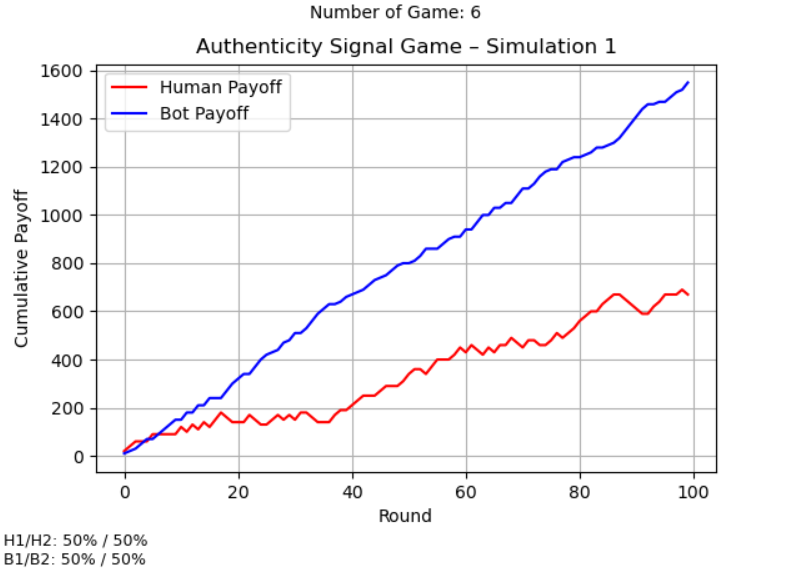
\includegraphics[width=1\textwidth]{Results Simulation/sim1_g6_50_50.png} % first figure itself
        %\caption{example of 1 of 50 games with the most ocurring phenomena}
    \end{minipage}\hfill
    \begin{minipage}{0.45\textwidth}
        \centering
        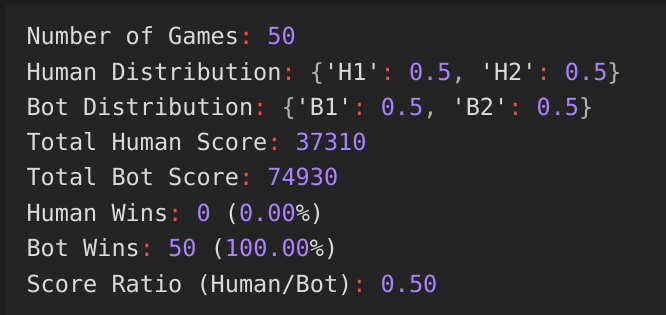
\includegraphics[width=1\textwidth]{Results Simulation//Results Stats/sim1_stat1.png} % second figure itself
        %\caption{second figure}
    \end{minipage}
\end{figure}
By increasing the probability for the human strategy H1 to 0.65 (and accordingly decreasing H2 to 0.35), we can state that the ratio of human payoff to bot payoff is roughly matched, despite the heavy deviations of the human payoff. This confirms that H1 is indeed the dominant strategy and pursuing H2 is not desirable at all. This is in contrary to the bot strategy distribution, as there is no dominant strategy and therefore changing this barely has any effect on human payoff.


\begin{figure}[H]
    \centering
    \begin{minipage}{0.50\textwidth}
        \centering
        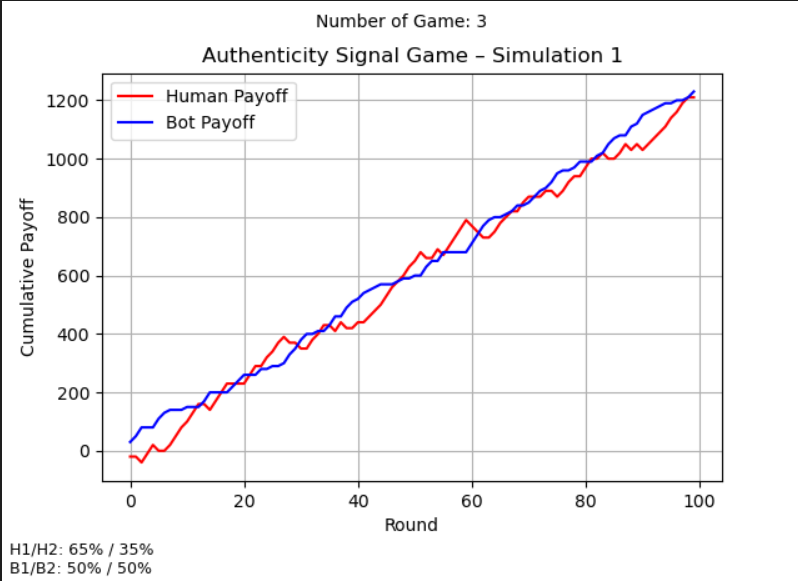
\includegraphics[width=1\textwidth]{Results Simulation/sim1_p2.png} % first figure itself
        %\caption{example of 1 of 50 games with the most ocurring phenomena}
    \end{minipage}\hfill
    \begin{minipage}{0.42\textwidth}
        \centering
        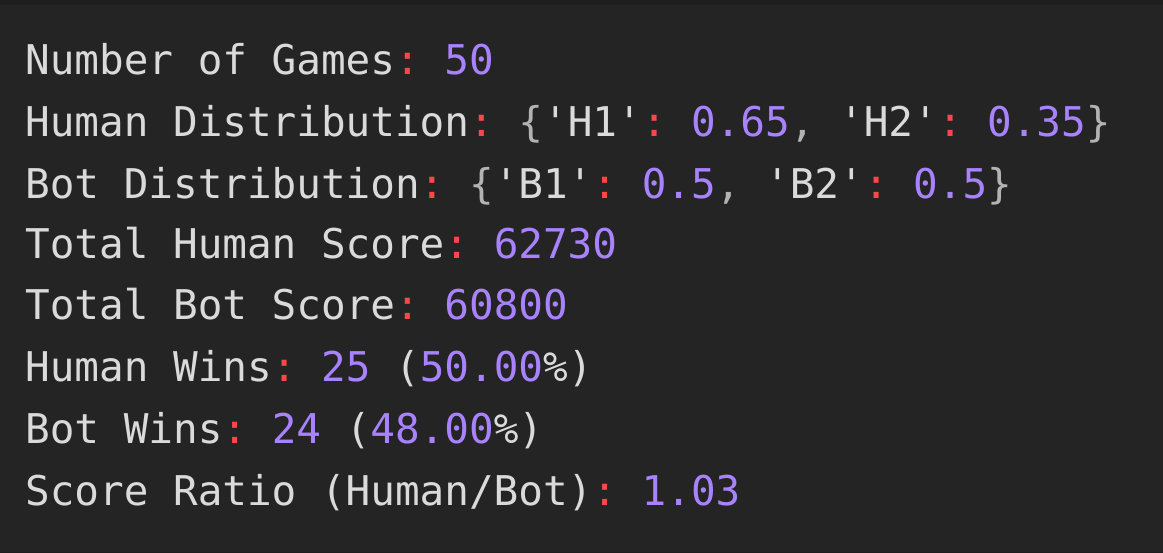
\includegraphics[width=1\textwidth]{Results Simulation/Results Stats/stats_sim1_p2.png} % second figure itself
        %\caption{second figure}
    \end{minipage}
\end{figure}

%\newpage

\subsection{Game with Penalties (Simulation 1.5)}
When running Simulation 1.5 with the default parameters, that is, a 50/50 distribution of both strategies for both B1/B2 and H1/H2, as well as a penalty strength/weight of 2 and a report probability of 0.3, we receive games with primarily the following phenomena:

\begin{figure}[H]
    \centering
    \begin{minipage}{0.55\textwidth}
        \centering
        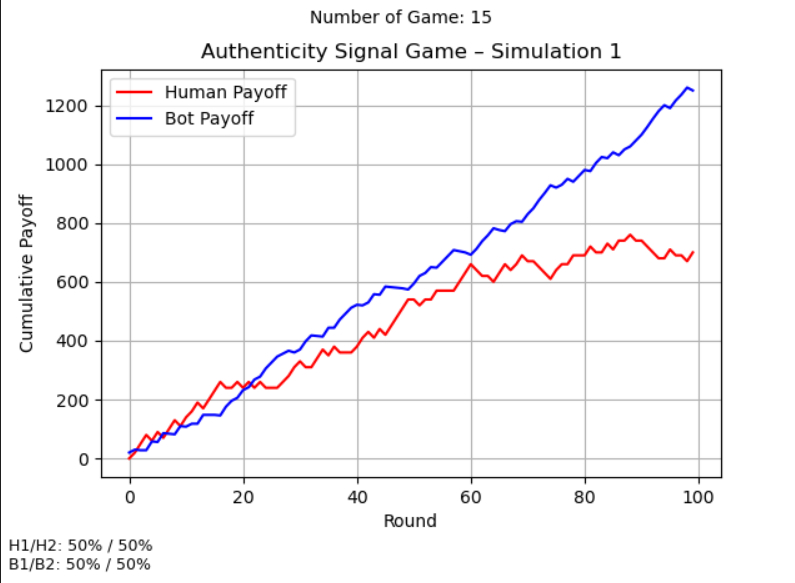
\includegraphics[width=1\textwidth]{Results Simulation/sim1_5_p1.png} % first figure itself
        %\caption{example of 1 of 50 games with the most ocurring phenomena}
    \end{minipage}\hfill
    \begin{minipage}{0.45\textwidth}
        \centering
        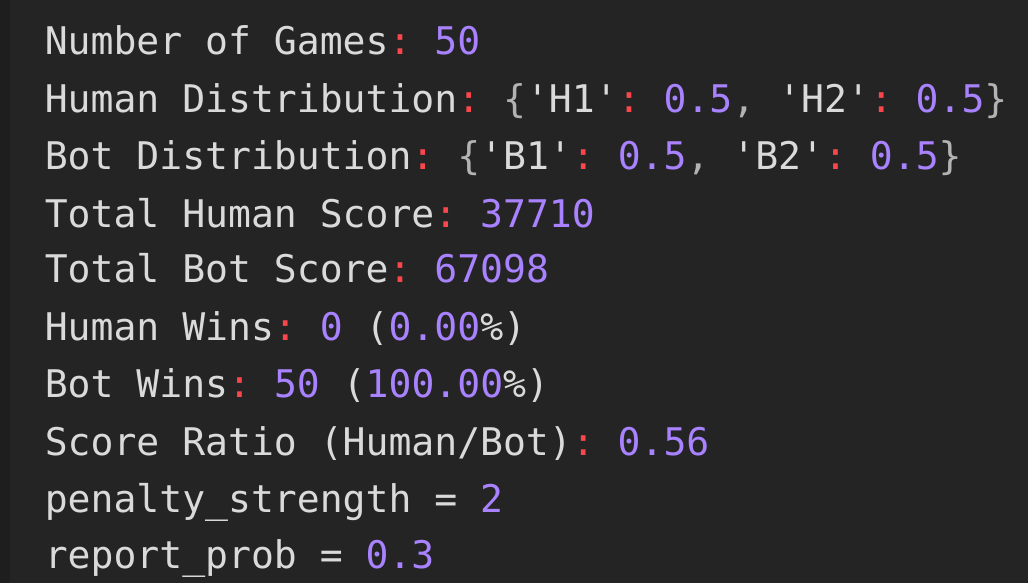
\includegraphics[width=1\textwidth]{Results Simulation/Results Stats/stat1_5_p1.png} % second figure itself
        %\caption{second figure}
    \end{minipage}
\end{figure}



The behaviour is very similar to the first simulation where both human and bot distribution was 50\%, however there is an increase in payoffs for humans, with sometimes 1 or even 2 games won by them (compared to 0 before). Although the bots' payout throughout the progression of the game is not constantly increasing, the long-term trend is still linear.
However, what occurs if solely the penalty\_strength increases? 
If the penalty\_strength is increased to 7, there is an increase in deviations, and both payoffs are not really stable, especially the human payoff. See, for example, an extreme game depicted in the figure below. There are cases where already early on in the game, dominance of one side is established and maintained. The threshold of almost equal payoffs between both entities (assuming the other parameters stay constant) is around 8.
The parameter for report probability has only minor affects for low penalty\_strength ($<$5). For higher penalty strengths, the report probability can, however, have a big influence as well and drastically increase human payoffs depending on the selection.


\begin{figure}[H]
    \centering
    \begin{minipage}{0.55\textwidth}
        \centering
        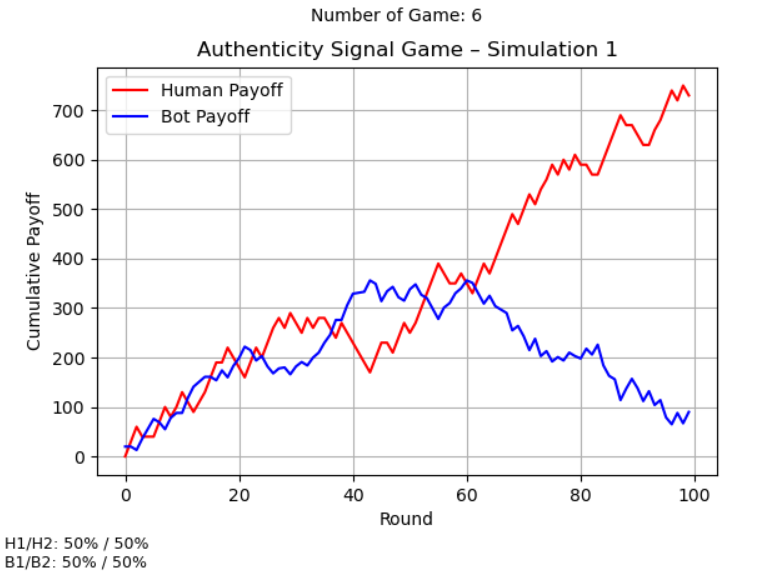
\includegraphics[width=1\textwidth]{Results Simulation/sim1_5_p2.png} % first figure itself
        %\caption{example of 1 of 50 games with the most ocurring phenomena}
    \end{minipage}\hfill
    \begin{minipage}{0.45\textwidth}
        \centering
        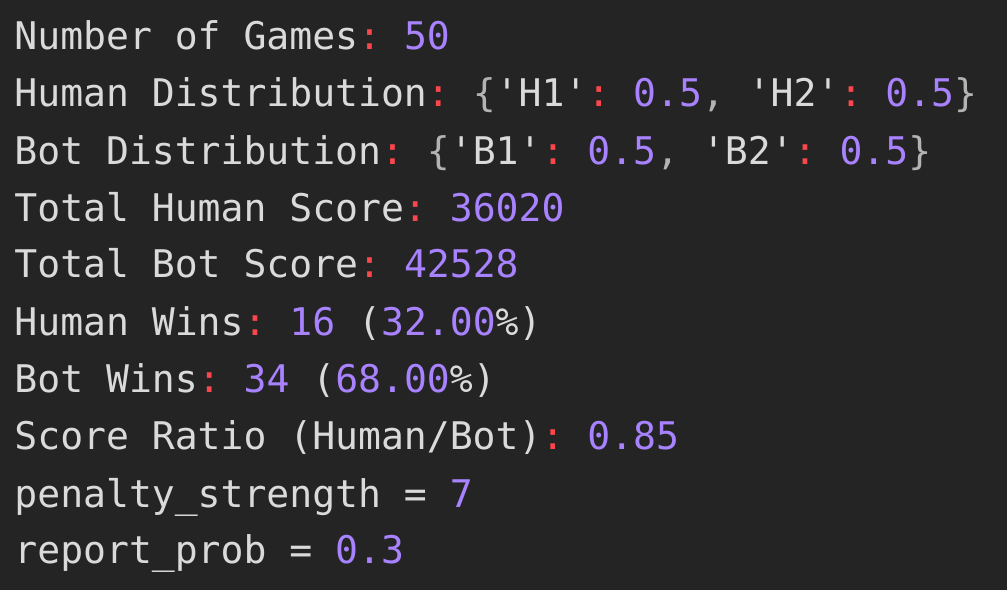
\includegraphics[width=1\textwidth]{Results Simulation/Results Stats/stat1_5_p2.png} % second figure itself
        %\caption{second figure}
    \end{minipage}
\end{figure}

%\newpage

\subsection{Game with Reports/Bans (Simulation 2)}

 By introducing blocking \& reports in Simulation 2, we notice that while the bot payoff does increase relatively linearly, occasionally it stagnates due to the blockages. Even in the 50/50 split of human and bot distributions with reporting and blocking, humans have a higher payoff compared to both simulations before.

\begin{figure}[H]
    \centering
    \begin{minipage}{0.55\textwidth}
        \centering
        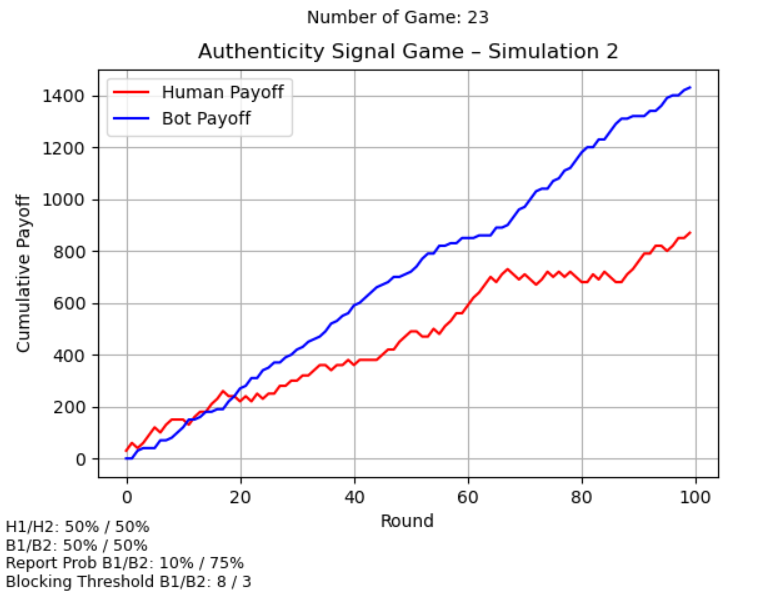
\includegraphics[width=1\textwidth]{Results Simulation/sim2_p1.png} % first figure itself
        %\caption{example of 1 of 50 games with the most ocurring phenomena}
    \end{minipage}\hfill
    \begin{minipage}{0.45\textwidth}
        \centering
        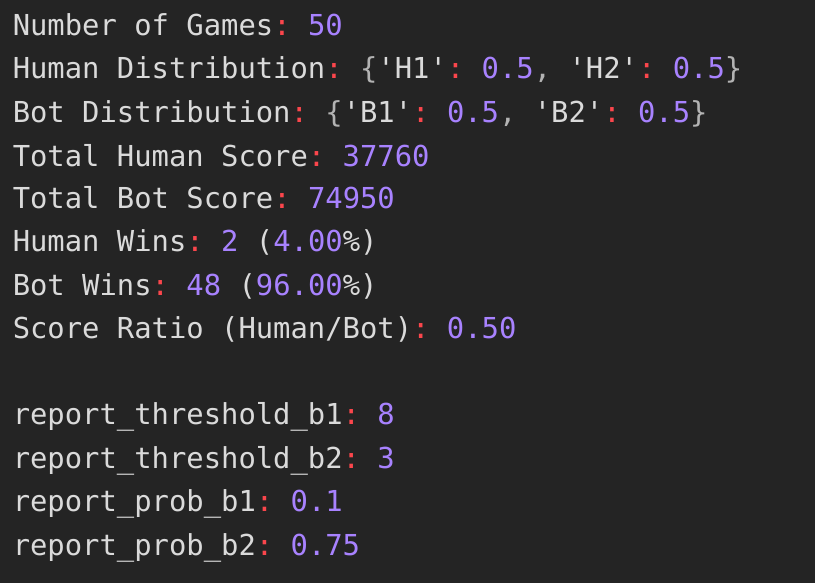
\includegraphics[width=1\textwidth]{Results Simulation/Results Stats/stat2_p1.png} % second figure itself
        %\caption{second figure}
    \end{minipage}
\end{figure}


 We can state that the threshold for even payoffs is around 65/35, i.e. 65\% of humans pursuing H1 and 35\% H2. It is important to note that in this case there is a high variance, i.e. the payoff of humans varies extremely. Even slight increases in the probability of the H1 strategy significantly increase human rewards compared to bots.

\begin{figure}[H]
    \centering
    \begin{minipage}{0.55\textwidth}
        \centering
        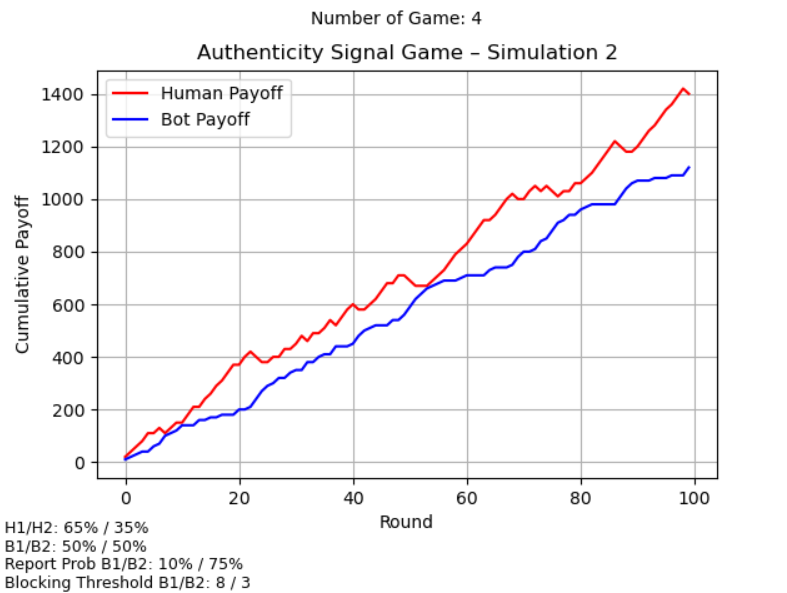
\includegraphics[width=1\textwidth]{Results Simulation/sim2_p2.png} % first figure itself

                %\caption{example of 1 of 50 games with the most ocurring phenomena}
    \end{minipage}\hfill
    \begin{minipage}{0.45\textwidth}
        \centering
        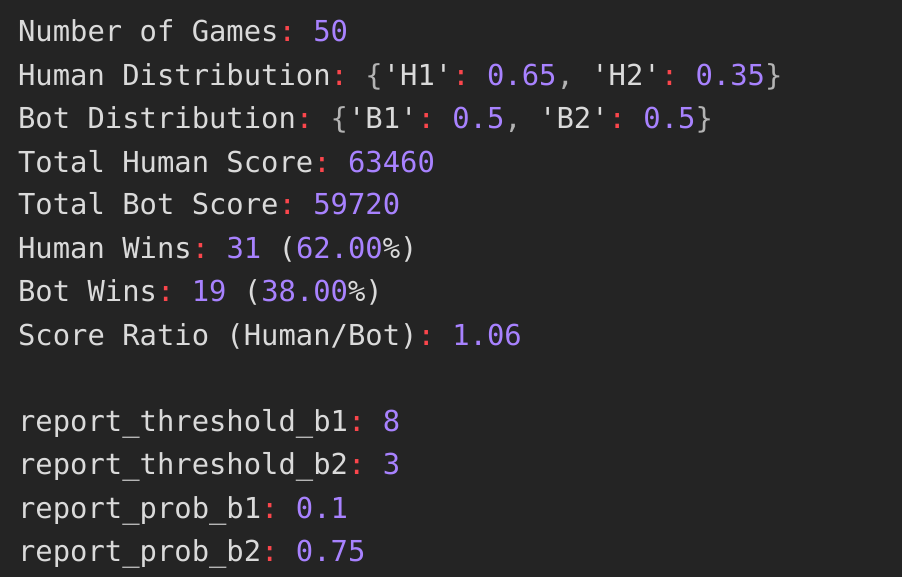
\includegraphics[width=1\textwidth]{Results Simulation/Results Stats/stat2_p2.png} % second figure itself
        %\caption{second figure}
    \end{minipage}
\end{figure}



 Finally, we can state that reporting obvious (strategy B2), as well as the not so obvious (strategy B1) bot activity leads to high payoffs for humans, due to the report threshold of both bot strategies. In addition, critical thinking and evaluation can make for a more authentic and human internet experience. In practice, there exist still a lot of edge cases, such as False Negatives or False Positives, that were attempted to be conveyed through probabilistic measures. Furthermore, the increase of LLM's makes it very difficult to discern the real from fake, especially if solely text is involved. 


\newpage

\section{Conclusion}%aaron
From our examination of the Dead Internet Theory through many domains of game theory and multiple simulations we have revealed interesting and central insights into the interactions between humans and bots on the Web. Our understanding of the factors that influence all this and the outcomes of multiple different games has been greatly improved. The results of the strategic game dynamics between AI and people have costly implications on the future of the Internet and the world. \\

Authenticity plays a huge role in creating trust of us humans. We rely on our judgement to decide whether the content is useful to us or not. And mass-produced AI products are not what we want, so bots try to mimic reality. This leads to a game of deception and detection, or, as we call it, the Authenticity Signal Game.\\

From our three simulations, we have concluded that both humans and bots can adapt strategically and rationally to get a positive payoff. However, there is no Nash equilibrium where a stable strategy exists for both parties. H1 is the dominant strategy for humans in all scenarios. In Simulation 1 the humans only get half the payoff to the bots and have zero chance of winning (for a 50/50 ratio of B1/B2 and H1/H2). It gets more interesting in Simulation 1.5, where the human has a small chance of winning (depending on how high the penalty\_strength is set), and their payoff increases. For the final simulation, the results show a staggeringly high payoff and win rate for humans, especially with increased reporting threshold and probability, i.e. choosing to inspect content and report a bot, if found, increases our chances of winning a lot.\\

It is never guaranteed that there is no manipulative behaviour happening from artificially generated content, but that all online news and posts are controlled by the government is rather improbable regarding our statistics. This questions the truthfulness of the Dead Internet Theory and its fundamentals. Although our results do suggest that external intervention may be necessary to shift the outcome of the game in favour of authenticity and us humans in the long run.\\

Next steps would be to extend our model to multiple players, different types of humans, various strategies, and possibly even learning behaviours of bots. Real-world data could definitely help to find patterns in this labyrinth of possible scenarios. Understanding these scenarios and their outcomes is essential for the web to remain a space where authentic, creative and genuine content thrives and no manipulative algorithms ruin our perception of reality.



\newpage
\section{Bibliography}
\bibliographystyle{unsrt}
\bibliography{references}


%possible an appendix with further code and craphs
\section{Appendix}
GitHub Repository: 
\nolinkurl{https://github.com/SmallPandaWorld/Contreversal_Game-Theory}

\end{document}
